\section{Neural Networks}\label{sec:neural_networks}
In this chapter, we will finally discuss the main topic of this thesis, \textit{Bayesian neural networks} (BNNs).
We will start off introducing the mathematical formalism of neural networks. 
We will then discuss the \textit{backpropagation} algorithm, which is the standard
algorithm used to compute the gradient of the model with respect to a specified loss. 
We will then finalize the chapter with how Bayesian learning of neural networks work. 
Fortunately, most of the groundwork is already laid, so we need only a mathematical description of the model and a Bayesian interpretation of it. 
We will stay general and assume a set of inputs $x \in \mathbb{R}^p$ and corresponding targets $y \in \mathbb{R}^d$. 
These serve as the training data on which the neural network is trained.
We will adopt the terminology used by the TensorFlow framework \cite{tf} to help make the
transition from mathematics to code easier. 

\subsection{Basic Mathematical Structure}
A neural network is most generally defined as a non-linear function $f : \mathbb{R}^p \to \mathbb{R}^d$ built up as follows.
\begin{itemize}
    \item A set of $L$ layers. Consider the $\ell$'th layer. It consists of $n_\ell$ nodes all of which has a one-to-one correspondence to a real number. 
    The conventional representation is with a real-valued vector $a^\ell \in \mathbb{R}^{n_\ell}$ called the \textit{activation} of layer $\ell$.
    \item For convenience, the layer with $\ell = 1$ is often called the \textit{input layer} and the layer with $\ell = L$ is
    referred to as the \textit{output layer}. The layers in between for $\ell = 2, ..., L-1$ are called the \textit{hidden layers}. Although this distinction is merely conceptual and does not change the mathematics one bit, it provides useful categories for discussion later on.
    \item Each layer $\ell$ is supplied with a (possibly) non-linear function $\sigma_\ell : \mathbb{R}^{n_{\ell - 1}} \to \mathbb{R}^{n_\ell}$. In other words, it defines a mapping $a^{\ell-1} \mapsto a^\ell$. The complete neural network function can thus be expressed as
    \begin{equation}
        f(x) = \left(\sigma_L \circ \sigma_{L-1} \circ \cdots \circ \sigma_\ell \circ \cdots \circ \sigma_2 \circ \sigma_1\right)(x).
    \end{equation}
    \item To each layer, we assign a \textit{kernel} $W^\ell \in \mathbb{R}^{{n_\ell} \times {n_{\ell - 1}}}$ and a \textit{bias} $b^\ell \in \mathbb{R}^{n_\ell}$. Together, these parameters are called the $weights$ of layer $\ell$. 
    \item The complete set of neural network parameters $(W,b) \equiv \{(W^\ell, b^\ell)\}_{\ell=1}^L$ are called the weights of the network. They serve as the \textit{learnable} or \textit{trainable} parameters of the model.
    \item Finally, we introduce the \textit{logits} $z^\ell \in \mathbb{R}^{n_\ell}$ of layer $\ell$.
    \item The permutation of number of layers, number of nodes per layer and activation functions are collectively called the \textit{architecture} of the neural network. 
\end{itemize}
The activation in layer $\ell$ is computed through the recursive equation:
\begin{equation}\label{eq:nn_forward_pass}
    a_j^\ell = \sigma_\ell \left(\sum_k W_{jk}^\ell a_k^{\ell - 1} + b_j^\ell \right) \equiv \sigma_\ell(z_j^\ell), \qq{for} j = 1, 2, ..., n_\ell.
\end{equation} 
A special case of eq.~\eqref{eq:nn_forward_pass} applies to $\ell = 1$ where $a^0 = x \in \mathbb{R}^p$ is assumed. 

\subsection{Backpropagation}
The standard approach to train a neural network is by minimization of some loss function by employing the backpropagation algorithm \cite{backprop} to compute its gradient with respect to its trainable parameters recursively. The algorithm boils down to four equations.
Consider $\mathcal{L}$ as the loss function.
The first of the four equations quantifes the error in the output layer.
\begin{equation}\label{eq:backprop1}
    \Delta_j^L = \pdv{\mathcal{L}}{z_j^L}.
\end{equation}
The second equation allows us to compute the error at layer $\ell$ given we know the error at layer $\ell+1$,
\begin{equation}\label{eq:backprop2}
    \Delta_j^\ell = \left(\sum_k \Delta_k^{\ell+1}W_{kj}^{\ell+1}\right)\sigma_\ell'(z_j^\ell).
\end{equation}
The final two equations relate these errors to the gradient of the loss function with respect to the model parameters. For the kernels, we have
\begin{equation}
    \pdv{\mathcal{L}}{W_{jk}^\ell} = \pdv{\mathcal{L}}{z_j^\ell}\pdv{z_j^\ell}{W_{jk}^\ell} = \Delta_j^\ell a_k^{\ell-1}.
\end{equation}
For the biases, the gradients are
\begin{equation}
    \pdv{\mathcal{L}}{b_j^\ell} = \pdv{\mathcal{L}}{z_j^\ell}\pdv{z_j^\ell}{b_j^\ell} = \Delta_j^\ell.
\end{equation}

With these four equations, we can fit the neural network using minimization techniques such as stochastic gradient descent or more complex methods such as ADAM (pages 13-19 in \cite{ml_for_physicists}). 
Although not the focus of this thesis, we might use these methods in conjunction with HMC to speed up convergence to the stationary distribution. Furthermore, the computation of gradients in combination with
HMC or NUTS is achieved with the backpropagation algorithm.
\begin{comment}

\subsection{Loss Function for Regression}
In this thesis, we are concerned with regression tasks. The activation function of the final layer $\sigma_L$ is then just the identity function. The typical loss function chosen to solve regression tasks is the $L_2$-norm, which for a single output can be written as 
\begin{equation}
    \mathcal{L}(y, \hat{y}) = \frac{1}{2}\norm{y-\hat{y}}_2^2,
\end{equation}
where $\hat{y}$ denotes the model output and $y$ the ground-truth. Now, the model output in this case is $\hat{y}_j = a_j^L = z_j^L$. Therefore, 
\begin{equation}
    \Delta_j^L = \pdv{\mathcal{L}}{z_j^L} = a_j^L - y_j.
\end{equation} 

\end{comment}

We are now equipped to write down the backpropagation for a single datapoint. It's built up of a \textit{forward pass} which takes an input $x$ and applies the recursive eq.~\eqref{eq:nn_forward_pass} which produces a model prediction $\hat{y} = a^L$. The second part of the algorithm 
is the \textit{backward pass} which based on the prediction $\hat{y}$ and the target $y$, computes the gradients of the loss function $\mathcal{L}$ with respect to the model parameters. The forward pass of the neural network
is summarized algorithm \ref{algo:forward_pass}.
\begin{figure}[H]
    \begin{algorithm}[H]
        \caption{Backpropagation: Forward pass}\label{algo:forward_pass}
        \begin{algorithmic}
        \Procedure{ForwardPass}{$x$}
        \State $a_j^0 = x_j$ \qq{for} $j = 1,\ldots, p$ \Comment{Initialize input} 
        \For {$\ell=1,2,.., L$}
        \For{$j=1,2,.., n_\ell$}
        \State $a_j^\ell \leftarrow \sigma_\ell\left(\sum_k W_{jk}^\ell a_k^{\ell-1} + b_j^\ell \right)$
        \EndFor
        \EndFor
        \EndProcedure
        \end{algorithmic}
    \end{algorithm}
\end{figure}
\noindent The backward pass of the algorithm is stated in algorithm \ref{algo:backward_pass}.
\begin{figure}[H]
    \begin{algorithm}[H]
        \caption{Backpropagation: Backward pass}\label{algo:backward_pass}
        \begin{algorithmic}
        \Procedure{BackwardPass}{$\mathcal{L}, x, y$}
        \For{$j=1,2,\ldots, n_L$}
        \State $\Delta_j^L \gets \pdv*{\mathcal{L}}{z_j^L}$
        \State $\pdv*{\mathcal{L}}{b_j^L} \leftarrow \Delta_j^L$
        \State $\pdv*{\mathcal{L}}{W_{jk}^L} \leftarrow \Delta_j^L a_k^{L-1}$
        \EndFor
        \For{$\ell = L-1, \ldots, 1$}
        \For{$j = 1, \ldots, n_\ell$}
        \State $\Delta_j^\ell \leftarrow \left(\sum_k \Delta_k^{\ell+1}W_{kj}^{\ell+1}\right) \sigma'(z_j^\ell)$
        \State $\pdv*{\mathcal{L}}{b_j^\ell} \leftarrow \Delta_j^\ell$
        \State $\pdv*{\mathcal{L}}{W_{jk}^\ell} \leftarrow \Delta_j^\ell a_k^{\ell-1}$
        \EndFor
        \EndFor
        \EndProcedure
        \end{algorithmic}
    \end{algorithm}
\end{figure}
\noindent Note that for in all practical implementations in this thesis, we utilize \textit{automatic differentiation}
provided by TensorFlow to compute the gradients.

\subsection{Regularization in Neural Networks}
As discussed in chapter \ref{chap:bayesian_ml}, models with a large number of parameters are prone to overfit
training data and generalize poorly as a consequence. Thus one typically tack on an $L^2$-regularization term to the loss $\mathcal{L}_0$. 
Assuming that $\mathcal{L}_0$ is the RSS in eq.~\eqref{eq:rss}, the form of the full loss function for a neural network model becomes
\begin{equation}
    \mathcal{L} = \frac{1}{2}\sum_i \norm{\hat{y}^{(i)} - y^{(i)}}_2^2 + \frac{\lambda_W}{2}\sum_\ell \norm{W^\ell}_2^2 + \frac{\lambda_b}{2}\sum_\ell \norm{b^\ell}_2^2,
\end{equation}
where $\lambda_W$ and $\lambda_b$ are regularization strengths for the kernels and biases respectively. The $L^2$-norm $\norm{\cdot}_2$ is the standard Euclidean norm in the case of a vector. For a matrix, we mean the following. Let $A \in \mathbb{R}^{m \times n}$. The matrix norm $\norm{\cdot}_2$ is then given by \textit{Fröbenius norm}
\begin{equation}
    \norm{A}_2 = \sqrt{\sum_{i=1}^m \sum_{j=1}^n \abs{A_{ij}}^2}.
\end{equation} 

\begin{comment}
\section{Activation Functions (NEW)}
There are many common activation functions with various strengths used in modern neural networks. We shall briefly mention a few ones
for completeness.

\begin{table}[h]
    \centering
    \begin{tabular}{llll}
        \hline
        \multicolumn{1}{l}{Name} & \multicolumn{1}{l}{Function} & \multicolumn{1}{l}{Derivative} & \multicolumn{1}{l}{Figure} \\ 
        \hline
        Sigmoid & $\sigma(x)=\frac{1}{1+e^{-x}}$ & $\sigma'(x)=\sigma(1-\sigma)$  &  
        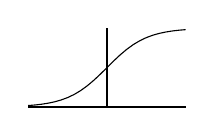
\begin{tikzpicture}[baseline={(0,0.2)}]
         \draw (-1,0) -- (1,0);
         \draw (0,0) -- (0,1);
         \draw plot[domain=-1:1,variable=\x] ({\x},{1/(1+exp(-4*\x))});
        \end{tikzpicture}\\
        \\
        tanh & $\sigma(x)=\frac{e^x-e^{-x}}{e^z+e^{-z}} $ & $\sigma'(x)=1-\sigma^2$   
        &  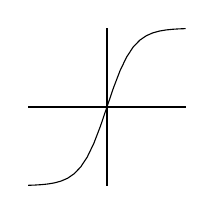
\begin{tikzpicture}[baseline={(0,0)}]
         \draw (-1,0) -- (1,0);
         \draw (0,-1) -- (0,1);
         \draw plot[domain=-1:1,variable=\x] ({\x},{tanh(3*\x)});
        \end{tikzpicture} \\
        ReLU & $\sigma(x) =\begin{cases}
        0 & ~\text{if}~ x<0 \\ 
        x & ~\text{if}~x \geq 0.
        \end{cases}$ & $\sigma'(x)=\begin{cases}
        0 & ~\text{if}~ x<0 \\ 
        1 & ~\text{if}~x > 0.
        \end{cases} $ & 
        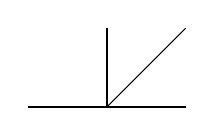
\begin{tikzpicture}[baseline={(0,0.5)}]
         \draw (-1,0) -- (1,0);
         \draw (0,0) -- (0,1);
         \draw plot[domain=-1:1,variable=\x] ({\x},{ifthenelse(\x<0,0,\x)});
        \end{tikzpicture}\\                      
    \end{tabular}
    \caption{Non-linear activation functions.}
    \label{tab:activationfct}
    \end{table}

\end{comment}

\section{Activation Functions}
There are many common activation functions with various strengths used in modern neural networks. We shall briefly mention a few ones
for completeness.

\subsection{Sigmoid and Tanh}
The sigmoid activation function is given by 
\begin{equation}\label{eq:sigmoid}
    \sigma(x) = \frac{1}{1 + \exp(-x)}.
\end{equation}
It was a very common choice in neural networks early, likely due to its simple derivative. It has a significant drawback, however.
Looking at eq.~\eqref{eq:sigmoid}, we can easily deduce that $\sigma(\pm \infty) = 0$, and since its derivative is of the form $\sigma'(x) = \sigma(1-\sigma)$,
the gradient computed during backpropagation vanishes if the input to the activation function as $\abs{x} \to \infty$. This significantly
hampers the progress during optimization. A popular alternative to the sigmoid function is the hyperbolic tangent given by 
\begin{equation}
    \tanh(x) = \frac{e^{2x} - 1}{e^{2x} + 1}.
\end{equation}
This function is very similar to sigmoid in the sense that its derivative vanishes
for inputs of large magnitude and so may suffer from the same issues as sigmoid does.


\subsection{ReLU}
To overcome the vanishing gradient problem, an activation function called the Rectifying Linear Unit (ReLU) became widely adopted, which is given by
\begin{equation}
    \sigma(x) = x^+ = \max(0, x).
\end{equation}
% The activation was found to perform well in deep learning back in 2011 \cite{relu} and has become widely adopted.


\subsection{Swish}
Recently, an activation function to replace ReLU was proposed in \cite{swish} known as \textit{swish} or SiLU which was shown to outperform ReLU in deep neural networks on
a number of challengig datasets. The activation function is given by
\begin{equation}
    \sigma(x) = x\cdot \text{sigmoid}(x).
\end{equation}


